\documentclass[unicode,10pt]{beamer}
\usetheme{ttipresentation}

\usepackage{geometry}
\usepackage{luatexja}
\usepackage{luatexja-fontspec}
\usepackage{graphicx}
\usepackage{multicol}

\setmainjfont{ipagp.otf}
\beamertemplatenavigationsymbolsempty
\geometry{a5paper,landscape}

\newcommand{\itemtitle}[1]{\textbf{#1}\\}
\newcommand{\fire}[1]{\textcolor{red}{\textbf{#1}}}
%\newcommand{\freeze}[1]{\textcolor{blue}{\textbf{#1}}}
\newcommand{\then}{\textcolor{ttiblue}{\textbf{⇒}}\hspace{1ex}}
\newcommand{\good}{\textcolor{orange}{\textbf{◎}}\hspace{1ex}}
\newcommand{\arrow}{\textcolor{ttiblue}{\textbf{→}}\hspace{1ex}}
\newlength{\mycolumnwidth}
\setlength{\mycolumnwidth}{0.495\textwidth}


\title{文書・文間及びカテゴリ間の関係を\\考慮したレーティング予測}
\institute{知能数理研究室}
\author{12056 外山 洋太}
\date{\today}



\begin{document}
\Large % HACK
\setbeamerfont{itemize item}{size=\Large} % HACK
\setbeamerfont{itemize subitem}{size=\Large} % HACK
\setbeamerfont{itemize subsubitem}{size=\Large} % HACK

\begin{frame}{パラグラフベクトルの目的関数}{}
  \begin{columns}
    \begin{column}{\mycolumnwidth}
      \begin{gather*}
        L = \sum_d L_d \\
        L_d = \frac{1}{T} \sum^{T}_{t = k + 1}
              \log p(w_t | w_{t-k}, ..., w_{t-1}), \\
        p(w_t | w_{t-k}, ..., w_{t-1})
            = \frac{e^{y_{w_t}}}{\sum_{w'} e^{y_{w'}}}, \\
        y = b + Uh(w_{t-k}, ..., w_{t-1}, d; W, D)
      \end{gather*}
    \end{column}
    \begin{column}{\mycolumnwidth}
      $d$:文書または文 \\
      $w_i$:文書または文中の$i$番目の単語 \\
      $W$:全ての単語のベクトルを含む行列 \\
      $D$:全ての文書または文のベクトルを含む行列 \\
      $T$:現在の文書または文に含まれる単語数 \\
      $k$:ウィンドウサイズ \\
      ウィンドウ:ある単語の周辺を表す区間 \\
      $p$:softmax関数により正規化された、
           文脈から現在の単語が導かれることの尤度 \\
      $h$:引数となる単語と文書または文のベクトルを結合した
           ベクトルを返す関数 \\
      %$y$:現在の単語とウィンドウ内の単語及び現在の文書または文から導出
    \end{column}
  \end{columns}
\end{frame}

\begin{frame}{文ベクトルの重み付け平均の式}{}
  \begin{columns}
    \begin{column}{\mycolumnwidth}
      \begin{gather*}
        \mathbf{t}_{i_{part}} = \sum_{i_{sent}}
                                \frac{w(x_{i_{part}}(i_{sent}))}
                                     {|\sum_{i_{sent}'}
                                      w(x_{i_{part}}(i_{sent}'))|}
                                \mathbf{s}_{i_{sent}}, \\
        x_{i_{part}}(i_{sent}) = \frac{i_{sent}}{\#sent - 1}
                                 - \frac{i_{part}}{\#part - 1}, \\
        w(x) = \begin{cases}
          \frac{1}{2} (\cos(\pi|x|) + 1) & \text{if $|x| \leq 1$} \\
          0 & \text{otherwise}
        \end{cases}
      \end{gather*}
    \end{column}
    \begin{column}{\mycolumnwidth}
      $\mathbf{s}_{i_{sent}}$:レビュー内の文ベクトル \\
      $\mathbf{t}_{i_{part}}$:重み付け平均された文ベクトル \\
      $i_{sent}$:レビュー内の文ベクトルのインデックス \\
      $i_{part}$:重み付け平均された文ベクトルのインデックス \\
      $\#sent$:レビュー内の文ベクトルの数 \\
      $\#part$:重み付け平均された文ベクトルの数
    \end{column}
  \end{columns}
\end{frame}

\begin{frame}{ニューラルネットワークの構成}{}
  \begin{itemize}
    \Large % HACK
    \item 活性化関数:シグモイド関数
      \Large % HACK
      \begin{gather*}
        \sigma(x) = \frac{1}{1 + e^{-x}}
      \end{gather*}
    \item 更新式:Adam
      \begin{itemize}
        \Large % HACK
        \item 重みについて更新された値を累積していき更新料が少ない
              重みを大きく更新する手法
        \item 確率的勾配降下法(SGD)より収束が早い
      \end{itemize}
    \item ドロップアウト
      \begin{itemize}
        \Large % HACK
        \item ある層においていくつかのニューロンの出力を
              確率的に0にする正則化の手法
        \item 実験では、入力層で0.2、中間層で0.5の確率
      \end{itemize}
    \item 重み減衰
      \begin{itemize}
        \Large % HACK
        \item ニューラルネットワークの重みの二乗和を目的関数に加え最小化する
              正則化の手法
        \item 実験では、係数5e-5で減衰
      \end{itemize}
  \end{itemize}
\end{frame}

\begin{frame}{実験結果}{}
  \begin{figure}
    \centering
    \caption{\large % HACK
             図. 各手法におけるのレーティングの正答率}
    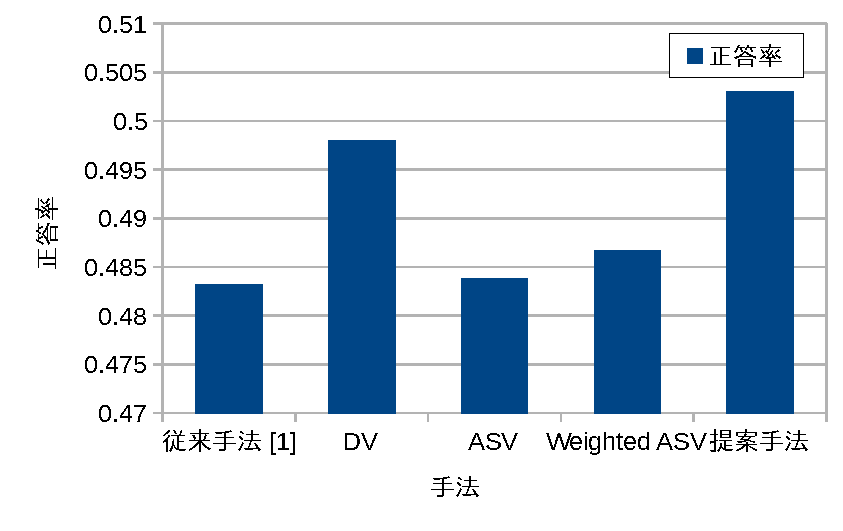
\includegraphics[width=0.8\linewidth]{fig/graph_of_accuracies_of_methods.pdf}
  \end{figure}
\end{frame}

\begin{frame}{実験結果}{}
  \begin{table}
    \centering
    \caption{\large % HACK
             表. 提案手法と従来手法におけるカテゴリ別のレーティングの正答率}
    \begin{tabular}{l | r r r r r r r}
      手法 & 立地 & 部屋 & 食事 & 風呂 & サービス & 設備 & 総合 \\
      \hline
      従来手法 & 0.4961 & 0.4706 & 0.5140 & 0.3973 & 0.4783 & 0.4265 & 0.5660 \\
      提案手法 & 0.5140 & 0.4984 & 0.5353 & 0.4347 & 0.5116 & 0.4479 & 0.5794 \\
    \end{tabular}
  \end{table}

  \begin{table}
    \centering
    \caption{\large % HACK
             表. 提案手法と従来手法におけるカテゴリ別のレーティングのRMSE}
    \begin{tabular}{l | r r r r r r r}
      手法 & 立地 & 部屋 & 食事 & 風呂 & サービス & 設備 & 総合 \\
      \hline
      従来手法 & 0.97 & 0.97 & 1.53 & 1.27 & 0.94 & 0.95 & 0.81 \\
      提案手法 & 0.88 & 0.88 & 0.93 & 1.03 & 0.86 & 0.90 & 0.73 \\
    \end{tabular}
  \end{table}
\end{frame}

\begin{frame}{実験結果}{}
  \begin{figure}
    \centering
    \caption{\large % HACK
             図. 提案手法と従来手法におけるカテゴリ別のレーティングの正答率}
    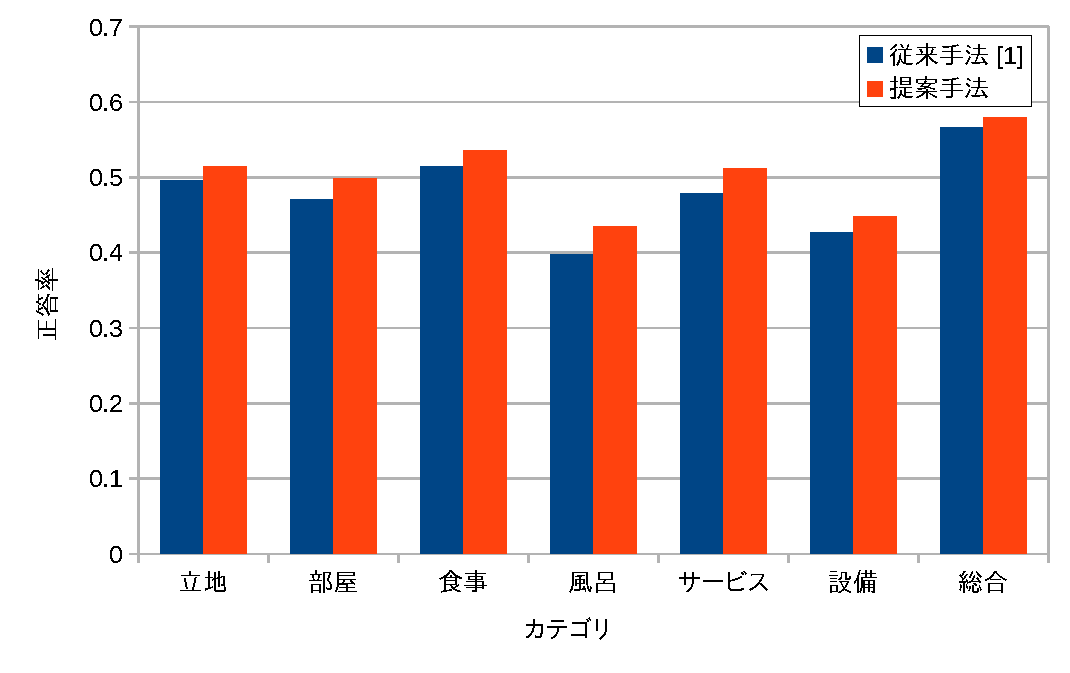
\includegraphics{fig/graph_of_accuracies_per_category.pdf}
  \end{figure}
\end{frame}

\begin{frame}{実験結果}{}
  \begin{figure}
    \centering
    \caption{\large % HACK
             図. 提案手法と従来手法におけるカテゴリ別のレーティングのRMSE}
    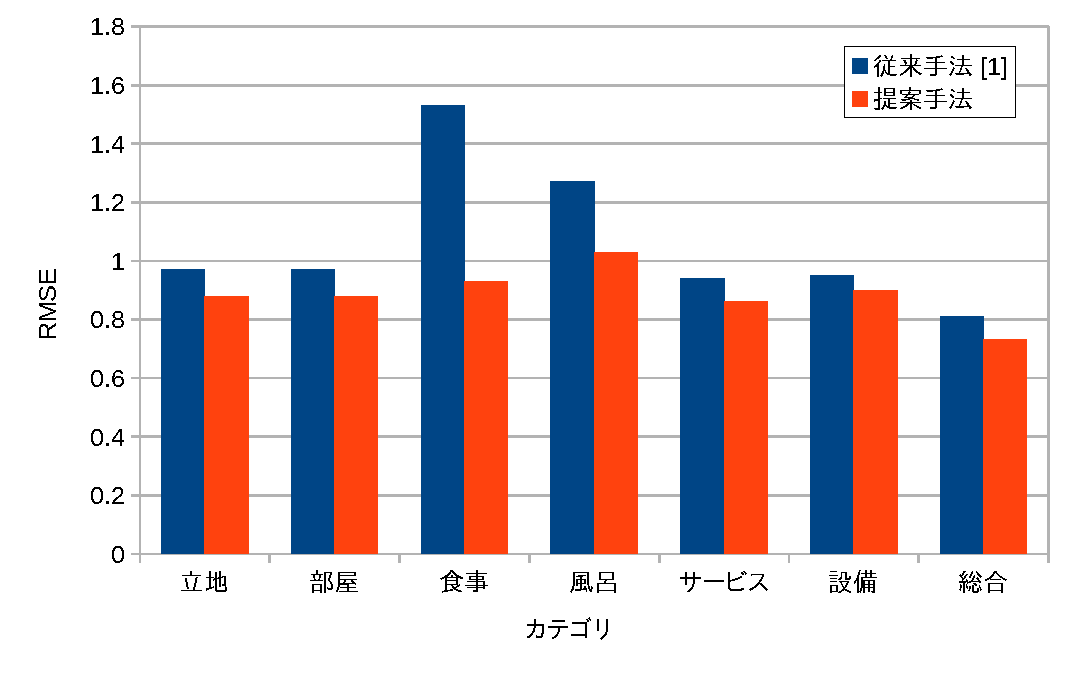
\includegraphics{fig/graph_of_rmses_per_category.pdf}
  \end{figure}
\end{frame}

\end{document}
